\documentclass[10pt]{article}

\usepackage[utf8x]{inputenc}
\usepackage[spanish, mexico, activeacute]{babel}
\usepackage{amssymb}
\usepackage{amsmath}
\usepackage{graphicx}
\usepackage[pdfstartview=FitH, pdftex, colorlinks=true]{hyperref}

\setlength{\topmargin}{0.0in}
\setlength{\oddsidemargin}{0.33in}
\setlength{\textheight}{8.0in}
\setlength{\textwidth}{6.0in}

\title{Plan de trabajo \\ {\large Trabajo de investigación
    para la materia de Métodos Analíticos} }

\author{Kael Huerta Acuña\footnote{
  \href{mailto:kaelhuerta@gmail.com}{kaelhuerta@gmail.com} }
  \qquad Alfredo Garbuno Iñigo\footnote{
  \href{mailto:alfredogarbuno@gmail.com}{alfredogarbuno@gmail.com} }\\
    {\small Maestría en Ciencia de Datos} \\
    {\small  Instituto Tecnológico Autónomo de México}}

\date{26 de febrero 2014}


\begin{document}

\maketitle

\begin{abstract}
Propuesta de proyecto final con plan de trabajo, entregables, base de datos y
contexto teórico.
\end{abstract}



\section{Introducción}
\label{sec:intro}

Se realizó un experimento en una exposición de arte en \href{https://dublin.sciencegallery.com/}{la galería de ciencias de Dublín}. En dicho experimento,
cada visitante a la galería contó con un dispositivo para obtener la proximidad
para con otros participantes. El resultado es una red dinámica en la que los
agentes entran en contacto unos con otros por intervalos de longitud variable
en distintos periodos de tiempo.\\



\section{Base de datos}
\label{sec:datos}

Cada visitante de la galería fue asignado con un dispositivo RFID ({\it Radio
Frequency IDentification}) para poder medir el contacto {\it cara a cara} que
tuvo a lo largo del día con los demás participantes. Que dos individuos hayan
estado en {\it contacto} implica que hayan estado por más de 20 segundos a una
distancia menor a 1.5 metros y de frente, pues el cuerpo humano actúa como
escudo para el envío y recepción de datos de los dispositivos.\\

Cada contacto entre dos individuos es almacenado con su respectivo instante
medido en términos de {\it timestamp} en formato {\it UNIX time}. Se cuenta
con 69 días de información de martes a domingo y el horario de la exposición
fue de 12 a 20 horas.\\

La base está conformada por 415,912 registros los cuales representan los contactos de los agentes que visitaron el museo. Cada registro cuenta con su etiqueta de tiempo. 159 individuos en promedio al día. Los agentes interactúan de tal forma que tenemos en promedio 6,030 contactos, los cuales definen en promedio 645 relaciones en un día promedio. 

\begin{figure}[!h]
\centering
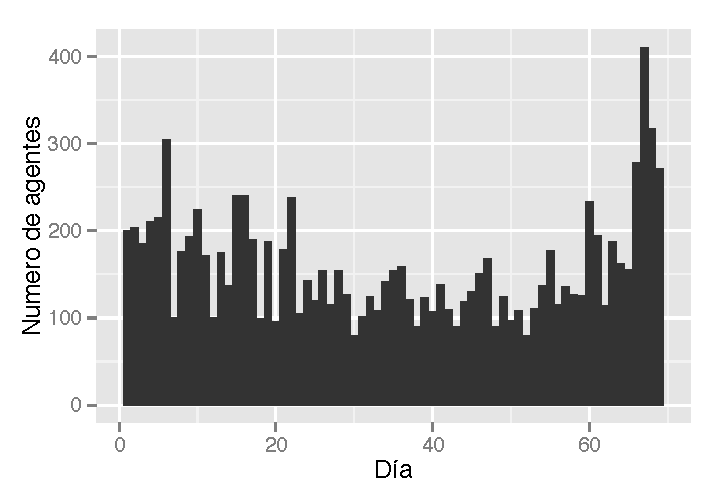
\includegraphics[width = .48\textwidth]{../Figs/agentes.pdf} 
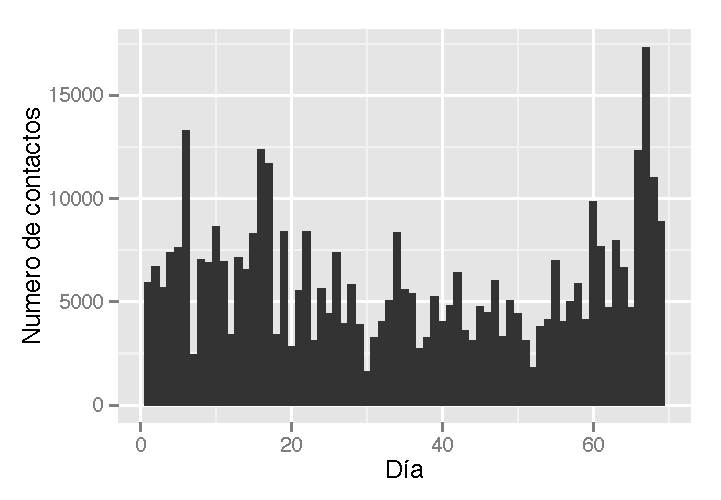
\includegraphics[width = .48\textwidth]{../Figs/contactos.pdf}\\
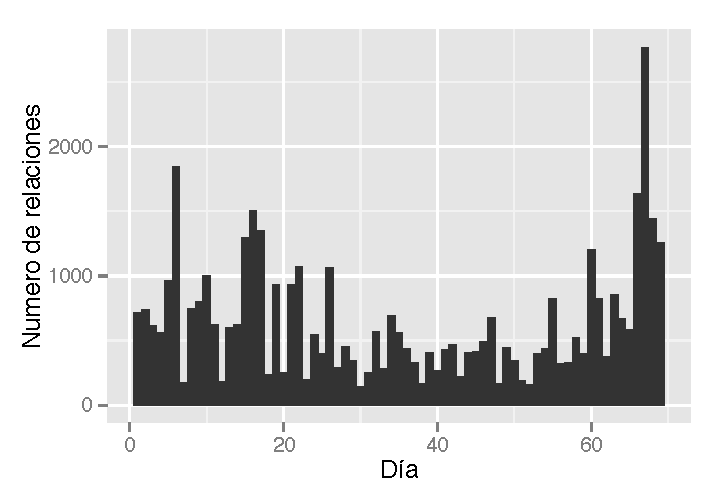
\includegraphics[width = .48\textwidth]{../Figs/relaciones.pdf}
\end{figure}



\section{Contexto teórico}

Las relaciones que describen los datos dan lugar a fenómenos en redes
dinámicas. Por esto, aunado al estudio del comportamiento y la estructura
de la red, el proyecto comprende la inmersión en temas de métricas temporales y
evolución de patrones a través del tiempo.\\

Anexo a lo ya descrito, se evaluará la posibilidad de incorporar el estudio de
transmisiones de enfermedades o contagio.



\section{Plan de trabajo}
\label{sec:plan}

La investigación se llevará a cabo de la siguiente manera:

\begin{itemize}
 \item {\bf Investigación teórica}. Incluye lectura de artículos, aprendizaje
  de los temas a continuación descritos y resúmenes.
  \begin{itemize}
   \item Osciladores
   \item Métricas en redes temporales
   \item Perfiles de comportamiento 
   \item Contagio\footnote{Pendiente por evaluar.}
  \end{itemize}
 \item {\bf Pruebas prácticas}. Comprende evaluar los métodos aprendidos con
 los datos disponibles.
  \begin{itemize}
   \item Exploración
   \item Análisis
   \item Visualización
  \end{itemize}
 \item {\bf Reporte de resultados}. Contempla el reporte y la presentación final.
  \begin{itemize}
   \item Hipótesis
   \item Supuestos
   \item Validación
   \item Conclusiones
  \end{itemize}
\end{itemize}

%\begin{figure}[t]
%  \begin{center}
%    \includegraphics[width=0.7\textwidth]{figura.pdf}
%  \end{center}
%  \caption{ Descripci\'on breve y clara del contenido de la figura.}
%  \label{fig:valles}
%\end{figure}



% archivo bibliografia.bib con todas las referencias.
% \bibliographystyle{siam}
% \bibliography{bibliografia}

\end{document}